\Chapter{Revision control}{}
\label{chap:Revision control}

\begin{quote}
\emph{``And then there's \texttt{git rebase --interactive}, which is a bit like \texttt{git commit --amend} hopped up on acid and holding a chainsaw---completely insane and quite dangerous but capable of exposing entirely new states of mind."} \\ \hspace*{\fill}---Ryan Tomayko
\end{quote}

A revision control system is perhaps the third most useful tool to a programmer after only the editor and compiler.
The idea is simple: you give a piece of software a description of recent changes you've made to your code, and that software will efficiently log the changes and description for you to view and optionally undo should you need to.
Written by Linus Torvalds and popularized by websites like \href{https://Github.com/}{Github}, Git is probablly the most widely used revision system around.
While a a full Git tutorial is far beyond the scope of this introduction, knowledge of a few basic commands can potentially save you a ton of time (and headaches!) down the road.

To get started, you'll want to install the \texttt{git}, \texttt{gitk}, and \texttt{git-gui} packages on Ubuntu. Next, let's assume you've created an \texttt{iccp/} directory with one file, \texttt{myProg.f90}, that already has some content. Navigate to the \texttt{iccp/} directory and type
\begin{verbatim}
$ git init
$ git add .
$ git commit -m ``Initial commit''
\end{verbatim}
This does a few things for you:
\begin{itemize}
  \item \texttt{git init} creates a git repository of \texttt{iccp/} by placing the current directory (and all sub-directories) under revision control.
    Any files and directories that get added to \texttt{iccp/} can be tracked as part of the current project.
  \item \texttt{git add .} adds every file's local changes to the \emph{staging area} or \emph{index}.
    The index tracks changes for you to inspect before they become an official part of the project history.
  \item \texttt{git commit -m ``Initial commit''} takes everything in the index and adds it to the history with the description ``Initial commit''.
\end{itemize}
You can add future changes in \texttt{myProg.f90} to the history in a similar way:
\begin{lstlisting}[style=prompt,nolol]
  $ git add myProg.f90              # or . to add everything
  $ git commit -m ``Fixed bug XYZ'' # use a msg appropriate for your changes
\end{lstlisting}
Similarly, you can check the current status of the index with \texttt{git status}. 
The output will display changes both staged and not staged in the index for the next commit, allowing you to tweak things as necessary.

If, after some bleary-eyed, hungover coding, you realize you've made a horrible mistake since your last commit, you can check a file's current state against the most recent history with
\begin{verbatim}
$ git diff <file>
\end{verbatim}
And to delete any changes you've made
\begin{verbatim}
$ git checkout <file>
\end{verbatim}
You can view the entire project history with the \texttt{gitk} program, including file diffs, commit messages, and authors. Similarly, \texttt{git gui} provides a handy interface for staging commits. You can write/ammend commit messages, see which files have changed and what files you've added to the index, push/pull to remote repositories, etc.

There are only a handful of ways to completely delete data from the repository once you've committed it\footnote{It's a good idea to avoid the more dangerous commands like \texttt{git rebase} and \texttt{git gc}. \textcolor{red}{\emph{Always}} think about commands before you run them!}, so unless you're \emph{really} trying to rewrite history your code is reasonably safe from git-mishaps.
That said, here are some tried and true tips to make the most of Git:
\begin{itemize}
  \item \textbf{Commit frequently}. The more commits you have, the more the history can help you.
    If you're trying to find a problem introduced in a new subroutine, it's much easier to search through ten lines of code you added in the past half hour than the 200 lines you added since Monday.
  \item \textbf{Commit \emph{logically}}. Commit complete logical units (like writing a function, fixing a bug, or formatting output) instead of just ``at the end of the day.''
    This greatly helps in reasoning about the development of your code---and thus undoing problems!
  \item \textbf{Use descriptive commit messages}. Messages like ``Fixed bug in force calculation'' and ``Implemented averaging function'' work far better than an endless series of ``nightly backup''s.
    If you can't easily reason about what's changed in your code, tracking the changes will do very little to help you.
  \item \textbf{Commit the bare minimum}. Only commit what's needed to recompile a functional program.
    Git just tracks the differences in files between commits to save space, but executables, output data, PDFs, images, etc. all require a totally new copy in the history every time they change (and that's frequently!)
    Tracking a \texttt{.gitignore} file with some simple patterns can automatically ignore files of a similar type.
  \item \textbf{Learn the advanced Git features}. Basic commits barely scratch the surface of Git's functionality.
    Branching lets you test drive changes in a copy of your code in an easily-reset sandbox, the network features let you not only backup code but also collaborate with other developers, and \texttt{git-bisect} can help you \emph{automatically} pinpoint exactly where and when a bug crept in.
\end{itemize}

You can find all of the example codes given in these notes at the \href{https://Github.com/cglosser/libICCP}{libICCP repository} on Github.
To use them, you'll want to \texttt{clone}\footnote{A clone is a complete local backup of the repository. It contains the entire project history and may itself be cloned and pulled from.} the repository with
\begin{verbatim}
$ git clone git@github.com:cglosser/libICCP.git
\end{verbatim}
You can then download any future changes to the repository with a \texttt{git pull} command inside the libICCP directory

Because of Git's popularity, the internet has a number of fantastic resources for learning to use it. \href{http://learn.Github.com/p/index.html}{Github Learning}, \href{http://git-scm.com/book}{Pro Git}, \href{http://think-like-a-git.net/}{Think Like a Git}, and \href{http://gitready.com/}{Git Ready} all offer very good tutorials and explanations.

\vfill

\begin{figure}[h!]
  \centering
  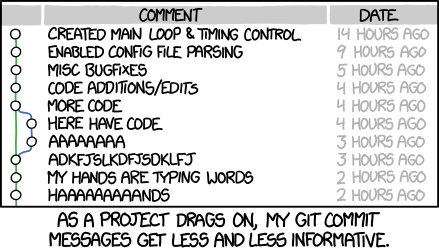
\includegraphics[width=0.4\textwidth]{figures/git_commit.png}

  \hspace*{\fill}---Randall Munroe (\href{https://xkcd.com/1296/}{XKCD})
\end{figure}
